
\subsection{Technologies}

Web clients were implemented on Node.js, with Vue and Element as javascript component libraries, and Crypto and CryptoJS as encryption tools.

\begin{itemize}
    \item \textbf{Runtime:} Node.js 6.13.4
    \item \textbf{Dependencies:} Vue 2.6.10; Element 2.13.0; Crypto 1.0.1; CryptoJS 2.1.3
\end{itemize}

Node.js is an asynchronous event-driven JavaScript runtime. With non-blocking calls, it is designed to build scalable network applications, which implements concurrency model\cite{nodejs}\cite{non-blocking}. Because of such a feature, a large number of open-source modules were built upon Node.js. To make use of these modules, Node.js was chosen to be used in this project.

Vue is a progressive framework for building user interfaces. The core library is focused on the view layer only, and is easy to pick up and integrate with other libraries or existing projects \cite{vue}. Element is a Vue 2.0 based component library. Most basic functions were implemented using Vue, especially when considering responsive data and components. To effectively construct a neat html page, components like chatting panel were pre-constructed to be rendered and inserted when needed. As an auxiliary tool for Vue, Element provided a variety of content-independent components together with fancy styles.

Crypto is an embeded crypto library of Node.js. We meant to utilize Crypto to implement all functionalities about encryption and decryption. However, AES related functions of Crypto did not work well with this project (it was missing some functions), so we turned to another library called CryptoJS. As a result, Crypto was used to generate Diffie-Hellman public and private keys during registration and to calculate shared secrets on initialising new chats, completing the functionality of key exchange. CryptoJS was used to do message encryption and decryption using AES with the previously computed shared secret key.


\subsection{Implementation}

Inspired by MVVM model, Vue provides an API for data binding. It is also called declarative rendering in \cite{vue}, because Vue pages preserve a section for data object storage that is realized by variable declaration, and binding is between these data objects and DOM objects. Besides, Vue data objects are written in a similar form as JSON, which means it easier using Vue to communicate with the Server. 

Web clients connect to the server through WebSocket in Web API, listening to predefined port, and communicating in the form of JSON requests and responses. If websockets are supported by a user's browser, the process of websocket initialisation done by \texttt{initWebSocket()} will be triggered once the pages are rendered. This is completed in \texttt{mounted()}, a predefined function of .vue files. In addition, the websocket connection will automatically close immediately after page destruction.

With constructed JSON requests, web clients use \texttt{this.websocket.send(this.request)} to forward it to the server. Since there is a latency to receive responses, web clients would get nothing when trying to parse JSON responses immediately after sending requests. Thus, a section named \texttt{watch} defined by Vue was exploited. It was to monitor any change on data objects and do reactions towards changes. only if responses are sensed and received from websocket will clients start to parse responses and do further actions.

Responses are stored in the data object called \texttt{response} with a sentence \texttt{this.response = event.data}. Once the change was detected, \texttt{watch} would parse the response with sentence \texttt{this.parsed\_response = JSON.parse(newR)} from JSON into Vue data objects. Afterwards, web clients can use the operator "\texttt{.}" to directly fetch related attributes that are consistent to the server. Figure \ref{tab:code-example} shows an example of how web clients deal with responses about messages from the server. It abstracts arguments from \texttt{parsed\_response} and pass them to \texttt{getNewText(sender, message)} to perform actual operations.

\begin{figure}[H]
 \centering
  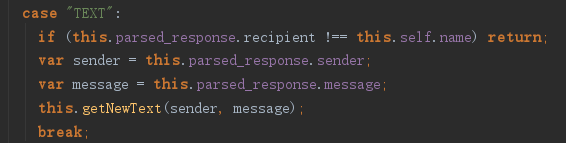
\includegraphics[width=0.8\textwidth]{images/code-example.png}
  \caption{Example of Operations on Responses}
  \label{tab:code-example}
\end{figure}

When using Vue components, we do not need to create DOM objects directly, such as \texttt{let newDiv = document.createElement("div")} but pass this job downwards. That is to say, if a new message was caught and corresponding UI was to be generated, the only thing we had to do was passing data to the pre-constructed component of message box. And it was the component itself that would decide how to present the data.

There are only two pages, \texttt{Signin.vue} and \texttt{Signup.vue}. The format of these files complied to Vue API.

As suggested by the name of \texttt{Signup.vue}, it was designed to handle registration of users. An agreement of registration constrains across both web and android was previously set, and details were described in \ref{android-implementation}. Web clients always check legality of input before constructing JSON requests of registration.

For \texttt{Signin.vue}, both login function and other main functions were integrated in one page. And users can only reach profile and chat information after successful login. Since functionalities of chat rely more on UI, reusable components were introduced in \texttt{Signin.vue}, so that redundant html codes could be omitted and replaced by particular function (i.e. for loop function).

\subsubsection{Components}

A table as follows shows the reusable components constructed in web clients.

\begin{table}[H]
\scriptsize
\begin{center}
\begin{tabular}{|c|c|}
\hline
\textbf{Components}             & \textbf{Description}                                                                                                                                                                                           \\ \hline
\texttt{single-chat.vue}                & \begin{tabular}[c]{@{}c@{}}A chat card in the contact list\\  indexing corresponding chat panel.\end{tabular}                                                                                                  \\ \hline
\texttt{group-chat.vue}                 & \begin{tabular}[c]{@{}c@{}}A group chat card in the contact list \\ indexing corresponding group chat panel.\end{tabular}                                                                                      \\ \hline
\texttt{single-chat-panel.vue}          & \begin{tabular}[c]{@{}c@{}}A chat panel showing decrypted messages\\  between two particular users. It may contain\\ \texttt{single-message-from-self.vue} and\\ \texttt{single-message-from-object.vue}.\end{tabular}           \\ \hline
\texttt{group-chat-panel.vue}           & \begin{tabular}[c]{@{}c@{}}A chat panel showing decrypted messages \\ among members of one particular group. \\ It may contain \texttt{single-message-from-self.vue} \\ and \texttt{single-message-from-group.vue}.\end{tabular} \\ \hline
\texttt{single-message-from-self.vue}   & \begin{tabular}[c]{@{}c@{}}A box showing one decrypted message together\\  with sending time from the authorised user.\end{tabular}                                                                            \\ \hline
\texttt{single-message-from-object.vue} & \begin{tabular}[c]{@{}c@{}}A box showing one decrypted message together \\ with sending time from the other in one chat.\end{tabular}                                                                          \\ \hline
\texttt{single-message-from-group.vue}  & \begin{tabular}[c]{@{}c@{}}A box showing one decrypted message from another\\  in one group chat, with time and related user name.\end{tabular}                                                                \\ \hline
\texttt{single-user-info.vue}           & \begin{tabular}[c]{@{}c@{}}A card shown in search user panel, specifying\\  user name, user email address and online status.\end{tabular}                                                                      \\ \hline
\texttt{single-group-info.vue}          & \begin{tabular}[c]{@{}c@{}}A card shown in search user panel, \\ specifying group name.\end{tabular}                                                                                           \\ \hline

\end{tabular}
\caption{Component Description}
\label{tab:component-table}

\end{center}
\end{table}

As shown in the above table, components can be nested (e.g. \texttt{single-chat-panel.vue} may contain \texttt{single-message-from-self.vue} and \texttt{single-message-from-object.vue}), which enhances their usability and convenience.The relation between components and UI and relation among components were depicted more clearly and intuitively in Figure \ref{tab:main-panel-of-user-chat} and Figure \ref{tab:main-panel-of-group-chat}.

\begin{figure}[H]
 \centering
  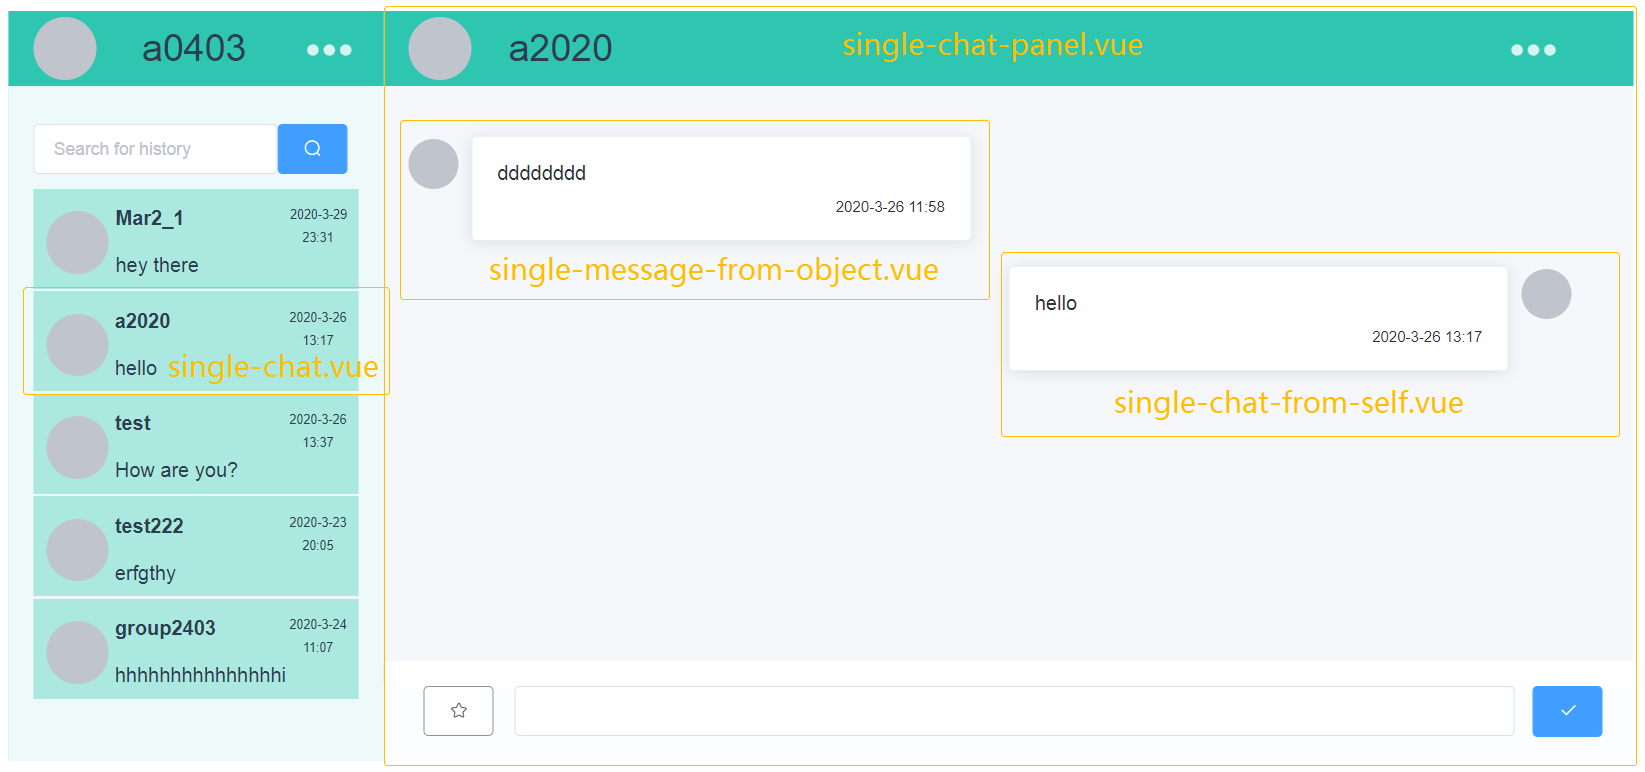
\includegraphics[width=1\textwidth]{images/user.png}
  \caption{Main Panel of User Chat}
  \label{tab:main-panel-of-user-chat}
\end{figure}

\begin{figure}[H]
 \centering
  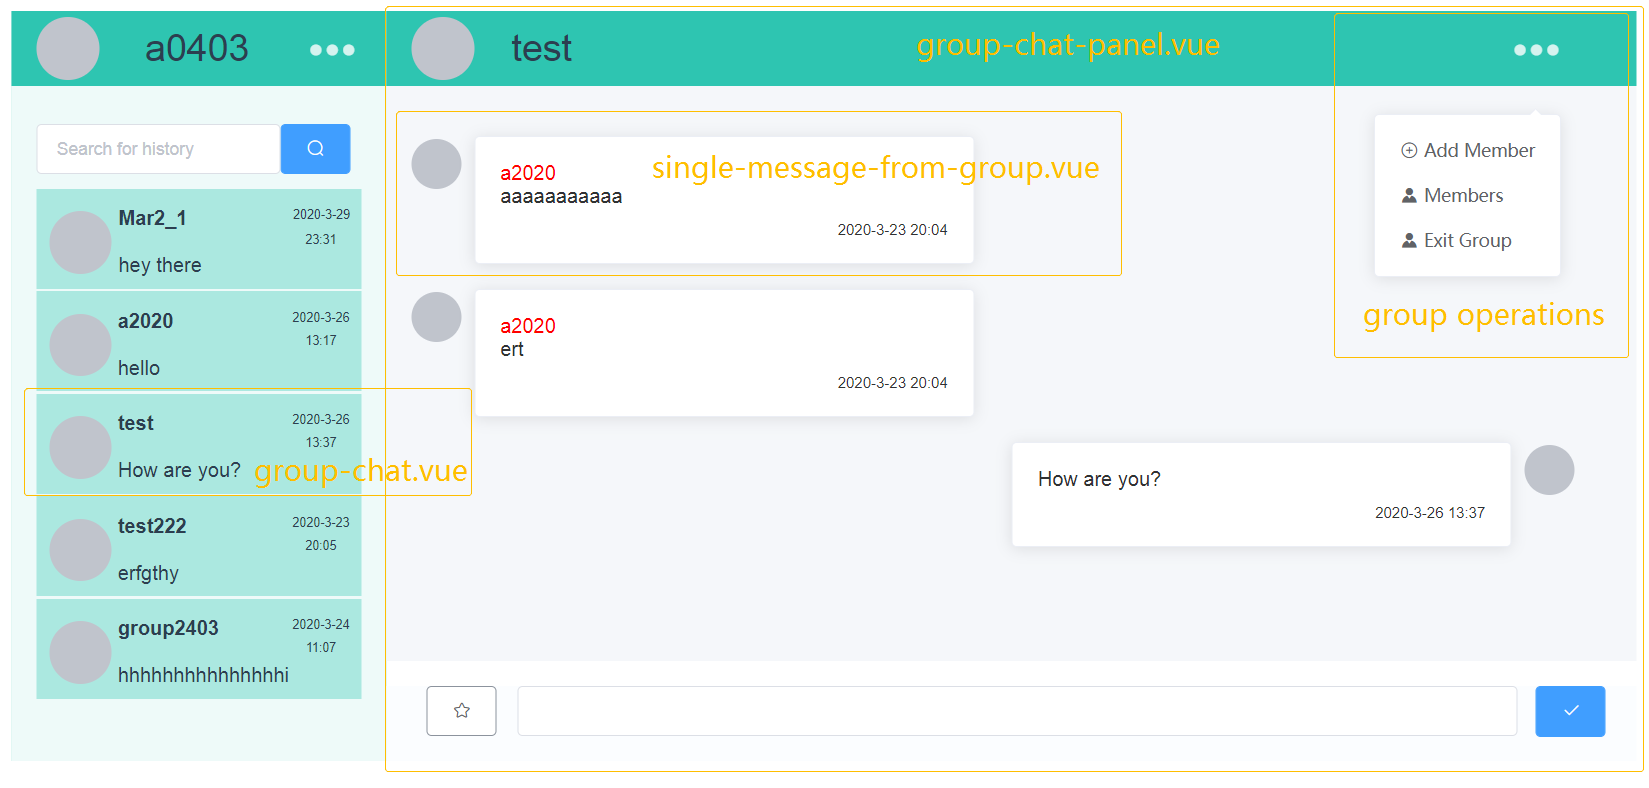
\includegraphics[width=1\textwidth]{images/group.png}
  \caption{Main Panel of Group Chat}
  \label{tab:main-panel-of-group-chat}
\end{figure}

There are more operations hidden in the "..." beside the user name, such as search users, search groups and create groups. Below it is a contact list, the list of users and groups that the concerned user can talk to. 

Each chat card in the contact list corresponds to one particular chatting panel and only one panel would be shown at a time. Since panels will be constructed and rendered previously once a new chat is created, it is fast to display them when needed without further loading. Upon one chat card, the last message content is presented as well as its sending time. Chatting panels present messages from last 24 hours and sorted temporally. For group chat messages, an extra information of sender user name is attached to each message box from others.

More group operations are in the "..." of group chatting panel. As shown in Figure \ref{tab:main-panel-of-group-chat}, they include adding group members, viewing current members and quitting the group.

There is no limit for requesting a chat, so an authenticated user can chat to anyone without their permissions. Every time when users log in, they need to search for other users and create a chat with them. Web clients will request for one-day chat history automatically but store no chat information on local storage. During this process, encryption techniques of DH key exchange and AES256 are used, which will be explained more in \ref{encryption}.

Upon both login and registration, passwords are hashed locally by MD5 to ensure confidentiality on networks.

\begin{figure}[H]
 \centering
  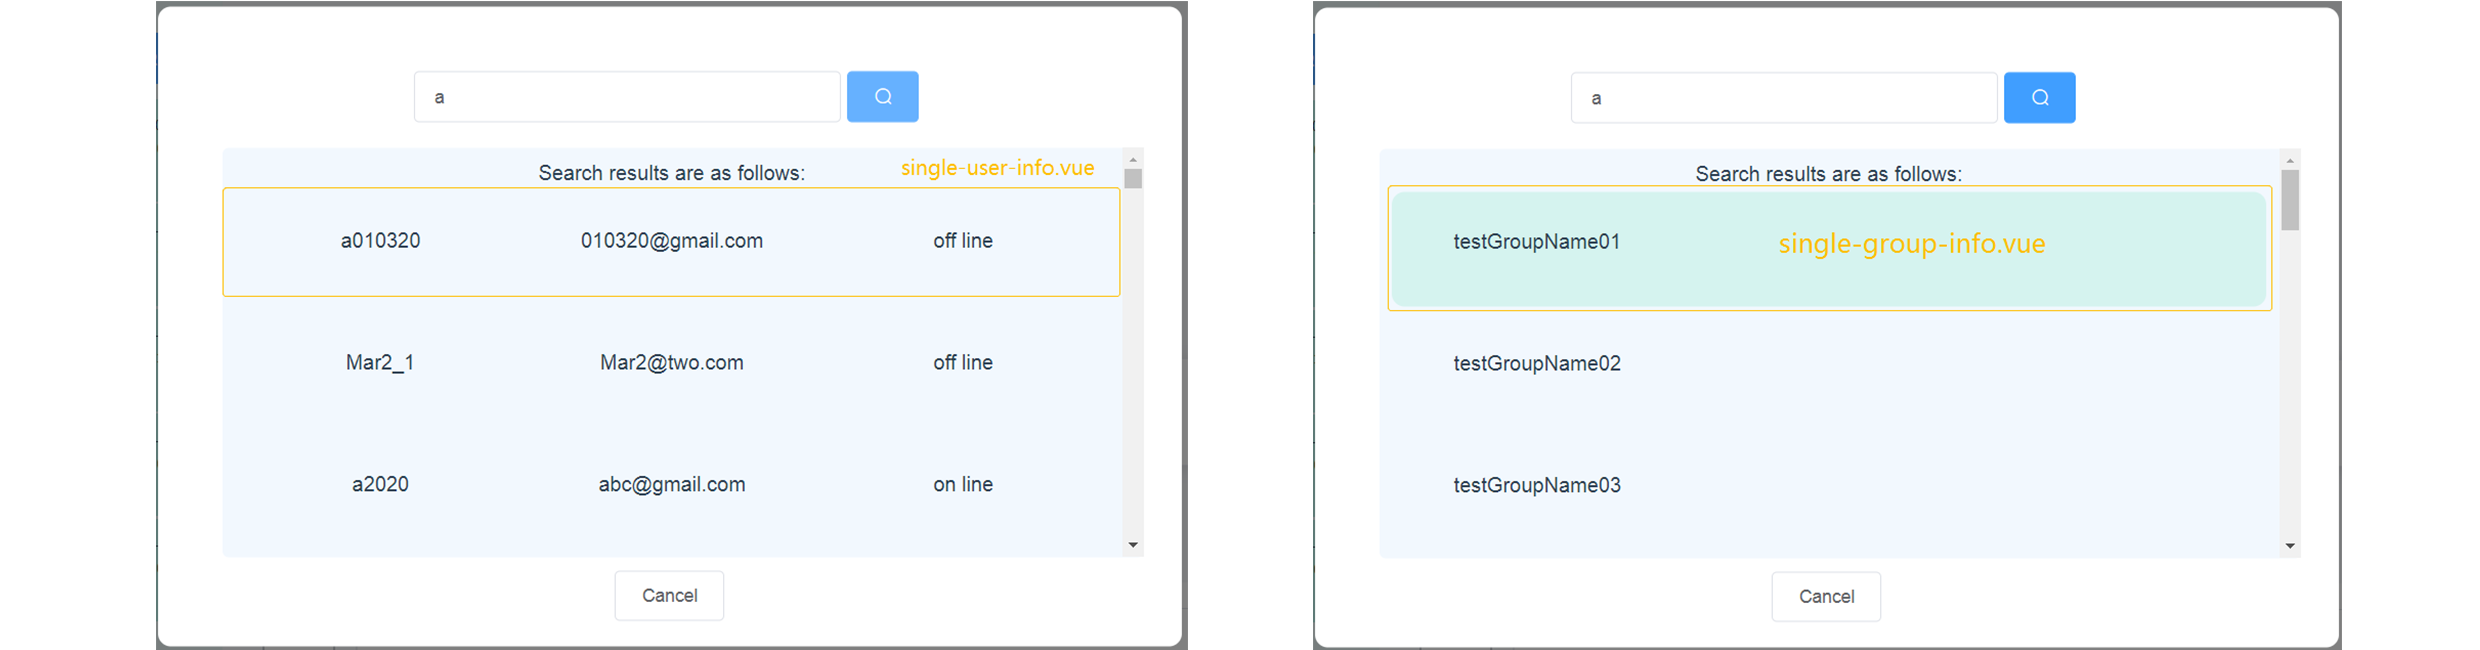
\includegraphics[width=1\textwidth]{images/search.png}
  \caption{Search Panels}
\end{figure}

Search user panel and search group panel can be triggered from the hidden more operations. For search user panel, the user is able to obtain basic information of concerned users. And the user can only create a new chat and start messaging from search user panel by clicking an interested information bar. On the other side, search group panel made use of a different policy. Search group panel only displays the list of searched group names, while the list of groups that the user is in are requested at the beginning after successful login. It is reasonable because the user may not be authorised to join every group. 

\subsection{Automation Testing}

The objective of testing here is to test functionality and usability of website. Automation testing is a testing technique, achieved by writing test scripts or using any automation testing tool to automate repetitive tasks and other testing tasks which are difficult to perform manually\cite{automation-testing}.

Like other testing, automation testing can be classified with respect to the phrase of testing: unit test, API test and UI based test. Among these tests, \verb|unit tests| are commonly run during the development phase. \verb|API tests| are run during the integration phase, before or after the UI layer is built for the application. \verb|UI based tests| are run to test the functionality and business logic of the application from the front end of the application\cite{automation-testing}.

Unit test and API test were implemented manually during the process of development and debugging. Only UI based test was run by automation scripts written with Selenium and Python. Testing file selenium-test.py is put under project directory \texttt{/frontend/src/test/}.

\subsubsection{Testing Environment}

Generally speaking, testing is supposed to be performed on various platforms in order to ensure completeness. However for the reason of limited devices and time, the testing was only finished under the following configuration.

\begin{itemize}
    \item \textbf{Operating system:} Windows 8.1
    \item \textbf{Browser:} Google Chrome 80.0.3987.149
    \item \textbf{Testing tools:} Selenium 6.13.4; JavaScript V8 8.0.426.27; Python 3.5.4
\end{itemize}

During the last year, Windows continued occupying the market of operating system of desktops and tablets\cite{desktop-tablet-os-market-share}. As for browsers, Google Chrome has been owning an overwhelming market share among other browsers from last year and made up 64.45\% in this February\cite{browser-market-share-worldwide}. Therefore, we can assume that such an environment configuration covers situations of the majority of users.

Selenium is an automation tool, providing extensions to emulate user interaction with browsers, a distribution server for scaling browser allocation, and the infrastructure for implementations of the W3C WebDriver specification\cite{selenium-project}. According to the survey sponsored by ToolsQA and conducted by Katalon and KMS Technology, Selenium is the most popular automation tool among over 100 tools reported, and a percentage of 84 of the respondents were using it\cite{automation-tools-survey}. In addition, Selenium provides good support for multiple platforms, browsers and programming languages. Thus, it is preferable to choose Selenium to be the automation tool used in this project.

\subsubsection{Test Cases}

With respect to the requirements we had implemented, the testing functions and test cases were planned to be constructed accordingly. Different from use cases, test cases are constructed to validate that software is working fine for each given instruction and yields required results. A simple list of test cases are classified as follows.

\begin{itemize}
    \item \textbf{Register:} to test validation rules, generation and storage of Diffie-Hellman key pairs and functionality of registration.
    \item \textbf{Login:} to test functionality of login and fetched public keys of other users.
    \item \textbf{User chat operations:} to test functionality of searching users, creating a new chat and message encryption with computed shared secret.
    \item \textbf{Group chat operations:} to test functionality of searching groups, creating groups and leaving groups.
\end{itemize}

\subsubsection{Test Results}

Due to time limit, not all of test cases were implemented as planned. Web clients perform good on reacting to registration of both legal and illegal request. Login inputs were not checked before requesting as registration does, but the functionality of login was implemented as required. Only users with private keys stored in local storage can login successfully. As for user chat operations, creating a new chat from search panel proved to work well after testing with no error by repeating searching users, entering search keywords and clicking a random user to start a chat. Since web clients could send encrypted messages and decrypt messages properly from other users, message encryption and decryption were believed to be implemented as console log did suggest messages in JSON requests were not plain text.

Automation testing of group chat operations were not performed yet, but successful cases were used manually to test related functionalities with positive result.

\subsection{Challenges and Drawbacks}

\begin{itemize}
    \item \textbf{Automation testing} Not all test cases were implemented; the automation test of web clients were only able to be performed locally. Though it was originally designed to cooperate with Travis CI, it failed due to the need to use local storage on clients to login and proceed further manipulation.
    \item \textbf{New message notification} There are still some bugs in terms of message notification. To be specific, notification would not appear when a user received a new message from another user not in the current chat list.
    \item \textbf{DH key generation} Although web clients can compute the same shared secret with DH keys generated by CryptoJS, there is a compatibility issue when cooperating with Android clients. The detail is that Web clients generate public and private keys with the same lengths, while Android clients using the \verb|java.security| library generate them with different lengths for some unclear reason.
    \item \textbf{Message encryption on group chat} Group message encryption remains to be implemented because of the difficulty of shared key computation among several users.
\end{itemize}